% !TEX TS-program = pdflatexmk
% !BIB TS-program = bibtex

\documentclass[12pt, a4paper, oneside]{book}
\usepackage{import}
\subimport{../}{preamble}
\ExecuteBibliographyOptions{articletitle=false}
\standalonetrue
\onehalfspacing
\begin{document}

\begin{singlespace}
\color{white}\chapter{Understanding and Applying Single Tip Plasmonics}
\label{ch:tip_plasmonics}
\end{singlespace}

%\AddToShipoutPictureBG*{ \AtPageUpperLeft{ \put(0,-255)
%{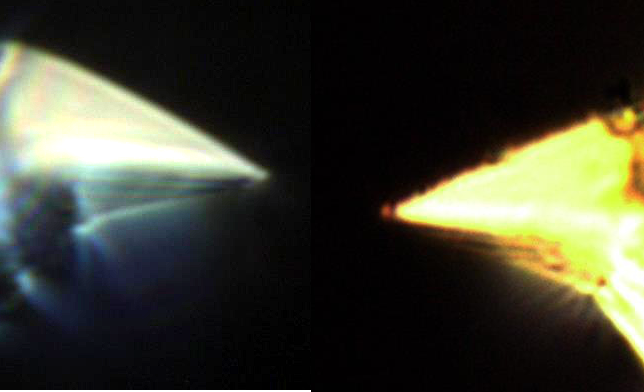
\includegraphics[width=\paperwidth, clip=true, trim=40 40 25 0]{data/chapter_cover.png}}
%}}
\AddToShipoutPictureBG*{ \AtPageUpperLeft{
\put(0,-250) {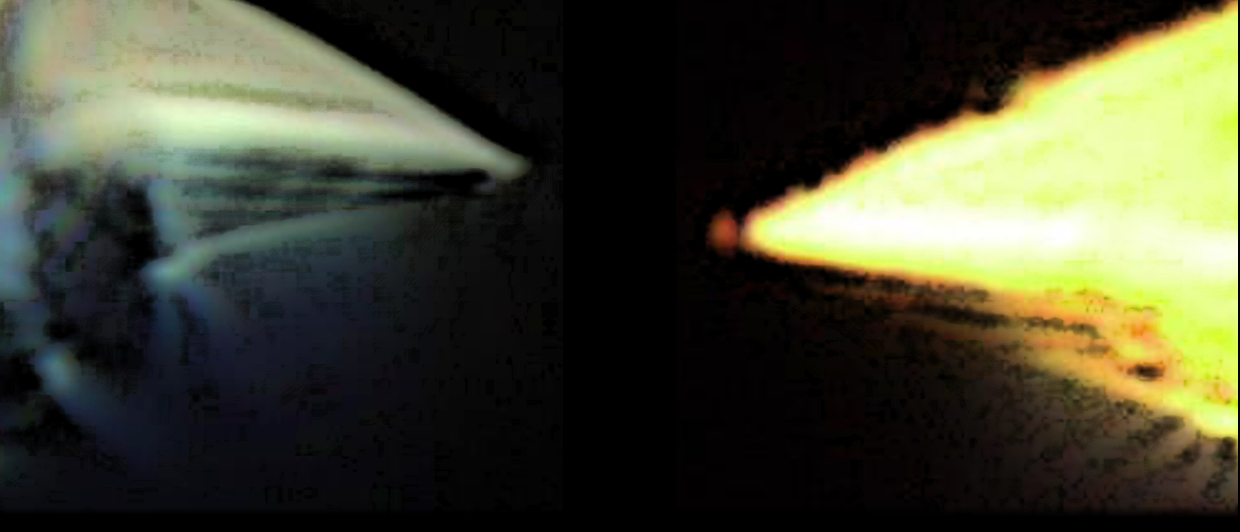
\includegraphics[width=\paperwidth]{../chapter_covers/tip_plasmonics_cover.png}}
\put(200,-5) {\begin{minipage}[t]{0.56\textwidth}\centering\singlespace\fontsize{9pt}{1em}\selectfont\color{white} Dark-field microscope images of a Pt and a spherical AuNP AFM tip. The AuNP tip apex plasmon strongly scatters red light.\end{minipage}}
}}


% Why do this
As discussed in the theoretical background (chapter \ref{sec:tip_literature}) only a small amount of work has been done to characterise and understand tips prior to applying them as optical nanoantennae. Understanding plasmons in tips, specifically those which can couple with far-field light, has been one of the main motivations of this project. A hyperspectral imaging technique is applied to laterally map light scattering from a tip with confocally localised spectra to infer a local optical response and better study different tips. Understanding this response at the apex of single tips is of importance in determining their effectiveness as near-field enhancers and in understanding their coupling behaviour in the presence of another tip. In this chapter the spectra of single tips is discussed, studying both sharp and spherical-tipped Au AFM probes, along with their application in Raman spectroscopy.

\subimport{./}{hyperspectral_imaging}
\subimport{./}{tip_plasmonics_understanding}
%\subimport{./}{nonplasmonic_tip_performance}
\subimport{./}{tip_plasmonics_applications}
%\subimport{./}{tuneable_raman}

\section{Conclusions}

%In conclusion, we have demonstrated a simple, fast method for the reliable growth of plasmonic spherical AuNP AFM tips. We showed this capability through measurements of dark-field scattering and SERS on controlled tip dimers at nanoscale separations.

Within this chapter it has been shown that spherical AuNP-tipped AFM probes are capable of supporting radiative LSPs in the red part of the visible spectrum that are not supported by the more conventional, sharp Au tips. These plasmons are clearly observed to exist at the apex of extended tip microstructures using scanning confocal hyperspectral imaging in the SDF microscope platform to locally probe the optical response. Broadband tuneable SERS is used to further confirm plasmonic behaviour in spherical Au tips. These techniques are ones that enable plasmon-dependent applications, such as TERS, to pre-screen nanostructured tips to better improve their reliability and reproducibility. The development of antenna-like plasmons in tips through nanostructuring, which readily couple to light without the need for momentum matching, is a step forward for TENOM. Furthermore, these modes determine what plasmonic phenomena are able to be experimentally observed, hence spherical tips can be used to dynamically investigate plasmonics.

\ifstandalone
\begin{singlespace}
\fontsize{8pt}{1em}\selectfont
\printbibliography[notcategory=fullcited]
\end{singlespace}
\fi

\end{document}